%% LyX 2.0.3 created this file.  For more info, see http://www.lyx.org/.
%% Do not edit unless you really know what you are doing.
\documentclass[english]{article}
\usepackage[T1]{fontenc}
\usepackage[latin9]{inputenc}
\usepackage{geometry}
\geometry{verbose}
\pagestyle{plain}
\setcounter{secnumdepth}{2}
\setcounter{tocdepth}{2}
\usepackage{array}
\usepackage{units}
\usepackage{graphicx}
\usepackage{setspace}
\onehalfspacing

\makeatletter

%%%%%%%%%%%%%%%%%%%%%%%%%%%%%% LyX specific LaTeX commands.
%% Because html converters don't know tabularnewline
\providecommand{\tabularnewline}{\\}

%%%%%%%%%%%%%%%%%%%%%%%%%%%%%% User specified LaTeX commands.
\usepackage{pbox}

\makeatother

\usepackage{babel}
\begin{document}

\title{Racecar: A Programming Language for Kids}

\maketitle
\tableofcontents{}


\section{Introduction}

Technology education for elementary school students is in its infancy.
Teachers are put in the unenviable position of trying to teach children
how to harness the potential of computers without actually knowing
how computers work and how to write computer programs. As a consequence,
many students are never exposed to computer programming and the algorithmic
critical thinking style that is critical to writing programs as well
as solving many other problems in life. Racecar is designed to solve
this problem by providing a language that is \emph{easy to teach},
even for non-experts; \emph{readable}, so parents can easily involve
themselves in their children\textquoteright{}s education; and \emph{engaging}
for 8 to 10-year-old children so they are motivated to experiment
and learn more about computers and programming, even outside of school.

In order to capture and maintain children\textquoteright{}s interest
in programming, Racecar is designed around a single goal: to write
a program that will navigate a car through an obstacle course. Students
will learn how to write programs that tell the car to move and turn
in specific sequences, a process that allows students to think about
concrete objects---an essential requirement for a language designed
for 8 to 10-year-olds---while they solve a prototypical problem of
the algorithmic style of thinking. More importantly, the programs
students write can be run using the accompanying application, which
shows the car as it executes the program\textquoteright{}s instructions
and navigates the obstacles. This immediate visual feedback is essential
for keeping students on task and excited about their progress. 


\subsection{What Problem Does Racecar Solve?}

Existing attempts to teach children about computer programming generally
utilize languages from one of three categories: graphical \textquotedblleft{}drag-and-drop\textquotedblright{}
programming, simplistic text programming (with graphical output),
and conventional programming languages. These various ideas each have
their drawbacks, and Racecar is designed to improve on all of the
positive aspects while minimizing the effects of the problems with
these techniques. In general, these languages fall short in one of
three categories: similarity to real-world programming (e.g. program
is not a text file), readability for non-experts, and a level of engagement
that captures children\textquoteright{}s interest. Racecar is designed
with these properties in mind, with the goal of making computer programming
extremely easy to teach in schools.


\subsection{Who Should Use Racecar?}

The intended users of this language are elementary school children
around the ages of 8 to 10, and their educators. Given that the purpose
of Racecar is to introduce these children to programming, no previous
experience is necessary. It is designed to be accessible and engaging
to children of all different interests and backgrounds. The scope
of the language is relatively small---it is clearly domain-specific---and
it is easy for a non-technical adult or teacher to pick up Racecar
as well; any elementary school teacher should be able to learn the
language quickly and to teach it effectively to others. Lastly, even
children\textquoteright{}s parents could learn how to write, or at
least read, Racecar programs to help on homeworks or independent projects
if necessary.


\subsection{Properties of Racecar}


\subsubsection{Easy to Teach}

Racecar is syntactically easy to understand so that instructors with
minimal knowledge of computer science concepts will be able to teach
the accompanying lessons and debug students\textquoteright{} programs
quickly. The lessons included with the language tutorial build on
each other, showing students that a complex task can be accomplished
by breaking the problem into manageable parts. Each lesson adds a
new movement (including \textquotedblleft{}drive straight\textquotedblright{}
and \textquotedblleft{}turn\textquotedblright{}) or programming concept
(including subroutines and looping/iteration) that can be integrated
into the previous lesson\textquoteright{}s program.


\subsubsection{Readable}

One of the biggest problems in the computer world is readability.
At every step of a computer science education, teachers and professors
beseech students to include whitespace, avoid long chains of function
calls, and comment as often as possible. However, it still seems that
people write indecipherable code that even experts have trouble understanding.
Language designers have tried to remedy this problem proactively by
writing \textquotedblleft{}readable\textquotedblright{} languages.
Existing readable languages include COBOL and Python. Both contain
syntactic constructs that are useful for programmers, yet degrade
readability. If you thought \textquotedbl{}OCCURS 12 TIMES\textquotedbl{}
means \textquotedblleft{}loop/repeat 12 times\textquotedblright{}
in COBOL, you\textquoteright{}d be wrong---it\textquoteright{}s a
declaration for a 12-element array! In Python (a vast improvement
from COBOL), many keywords and functions such as \textquotedblleft{}def,\textquotedblright{}
\textquotedblleft{}len,\textquotedblright{} and \textquotedblleft{}str\textquotedblright{}
are short, making them easy to type, but hard for non-experts to recognize.
Racecar strives to be readable even to non-technical students, teachers
and parents. For example, Racecar is a statically typed language,
and there are two primitive types: \textquotedblleft{}number\textquotedblright{}
and \textquotedblleft{}word.\textquotedblright{} No \textquotedblleft{}ints,\textquotedblright{}
\textquotedblleft{}floats,\textquotedblright{} or \textquotedblleft{}doubles\textquotedblright{}
are around to complicate things, and although \textquotedblleft{}string\textquotedblright{}
might be a more general term, \textquotedblleft{}word\textquotedblright{}
emphasizes the important difference between the data types more clearly
than \textquotedblleft{}string\textquotedblright{} does. All of Racecar's
keywords and constructs are designed with this kind of readability
in mind. Table $1$ demonstrates some examples of Racecar's readability.
\begin{table}[h]
\begin{tabular}{|c|c|c|>{\raggedright}p{0.2\textwidth}|}
\hline 
Concept & Python & Racecar & Comments\tabularnewline
\hline 
\hline 
Method declaration & $\mathtt{def\ myMethod(var1,\ var2):}$ & \pbox{5cm}{$\mathtt{define\ myMethod\ using\ var1}$\\$\mathtt{\ (number)\ and\ var2\ (word)}$} & Uses full words instead of abbreviations and punctuation\tabularnewline
\hline 
Iteration & $\mathtt{for\ i\ in\ range(5):}$ & $\mathtt{repeat\ 5\ times}$ & Uses simple, clear, intuitive keywords\tabularnewline
\hline 
Method invocation & \pbox{5cm}{$\mathtt{car.drive(direction.}$\\$\mathtt{FORWARD,\ 10)}$} & $\mathtt{drive\ forward\ 5\ steps}$ & Syntax is similar to OCaml and Haskell: no dots or parentheses required!\tabularnewline
\hline 
\end{tabular}\caption{Examples of Racecar syntax compared to Python syntax}


\end{table}



\subsubsection{Engaging}

The accompanying application will have a simple 2-D animation of a
car following the commands the student programmed. The ability to
control the outcome of an action, such as driving a car, is engaging
and teaches students to think creatively while still conforming to
rules. Navigating a car visually may be trivial, but Racecar will
show students that a precise definition of the car\textquoteright{}s
movement is necessary to achieve the desired outcome. The goal-oriented
nature of the lessons combined with frequent positive feedback coming
from the graphical application captures children\textquoteright{}s
attention. Accomplishing the complex goal at the end of the lesson
sequence is rewarding and builds confidence to tackle subsequent challenges.


\subsection{Similar Programming Languages}

There are a number of technologies available whose goal is to teach
children in elementary school to think algorithmically and programmatically.
One such \textquotedblleft{}language\textquotedblright{} is MIT\textquoteright{}s
Scratch platform, which presents a graphics-based language to children;
code is constructed using a drag-and-drop interface. However, physically
typing commands into a text editor is paramount in internalization
of language constructs, programming style, and procedural thinking.
Racecar\textquoteright{}s language and platform combines these approaches,
compelling children to write their programs in a normal text editor,
but then compiling it and importing it into an application where they
can see graphical output of their code.

Other approaches to teaching algorithmic thinking have taken the form
of games, completely abstracting away the idea of programming form
the user. For example, Armor Games\textquoteright{} Light Bot (http://cache.armorgames.com/files/games/light-bot-2205.swf)
gives children a platform on which to build small programs with a
limited number of instructions, forcing them to think in terms of
subroutines. Again, this platform, while certainly engaging, fails
to give children the irreplaceable experience of typing a procedure
word for word, the importance of which was discussed earlier.

Older technologies like LOGO incorporate true algorithmic thinking
and graphical output. However, LOGO\textquoteright{}s platform is
not as engaging as children have come to expect from modern software.
Furthermore, LOGO\textquoteright{}s language itself lacks human-readability
compared to Racecar, a feature that is particularly important in conveying
programmatic ideas and facilitating an easy transition into coding
for children.

Finally, platforms like Lego Mindstorms give children the ability
to program their legos to move, allowing creations like robots, self-driving
cars, etc. Hardware-based approaches, however, have fundamental limitations
in distribution. One set of legos can create only one robot at a time;
there is no such limitation with a purely software-based platform,
since, for example, a proud parent can send his child\textquoteright{}s
program to relatives without making them buy physical kits.


\section{Lesson Plans}


\subsubsection{Introduction: How to Use Racecar}

Racecar is a programming language that allows you to control the motion
of a virtual car on the computer screen. The following lessons are
designed to teach both you and your students to learn how to write
programs that tell the car to move in increasingly sophisticated patterns
and routines. Although at first you will only be able to drive in
a straight line, by the end of Lesson $10$ you will know how to drive
in any pattern you can think of and navigate around obstacles on the
screen! Before we get to the programming lessons, there are a few
things that you, the teacher, should be familiar with so that teaching
and helping your students to program is as easy as possible.

First, let's look at the Racecar application. It consists of a window
for writing Racecar code, a screen displaying the car and its surroundings,
and a few menus and buttons. The big GO button is what you click when
you want to run the program sitting in the program window. The STOP
button is how you stop a program that's running if you want it to
finish early. The other menus have the usual Save, Open, and Quit
buttons that you may be used to from other computer applications.

Second, here are some basic concepts in Racecar that are not exactly
programming concepts, but are still invaluable when writing code.
Racecar is case-sensitive, which means that the computer treats the
expressions like $\mathtt{drive}$ and $\mathtt{DRIVE}$ as two completely
different, completely unrelated words. Along the same lines, Racecar
will not fix your spelling, so be sure to check for typos as you write
your programs, as any typos will cause your program to not work as
expected. Names that you come up with in Racecar to represent numbers,
words, and actions (which are called \textquotedblleft{}variable names\textquotedblright{}
and \textquotedblleft{}function names\textquotedblright{}) cannot
have any spaces in them. A standard trick programmers use to keep
their names readable, even when they consist of more than one English
word, is called Camel Case: keep the first letter lowercase, and then
capitalize the first letter of every new word. For example, the phrase
\textquotedblleft{}You can write in Racecar\textquotedblright{} would
be formatted in Camel Case as $\mathtt{youCanWriteInRacecar}$. This
way, it is simple to see where the words begin and end even though
there are no spaces. Another important restriction on these variable
and function names is that they cannot be the same as Racecar's keywords.
In the language reference manual, Section 10 contains a list of all
of the keywords (reserved words) that would lead to ambiguity (and
hence errors) if they were used as variable or function names. 

Finally, we will share some important lessons about the human side
of computer programming. An important part of programming that is
not so obvious is that programs are supposed to be written so that
\emph{other people} can read them. That is, programs should not be
written so that the computer finds them easy to read, but rather so
that people find them easy to read. If we wanted programs to be easy
for computers to read, we would write in 1's and 0's! (In fact, that
was essentially how programs were written when computers were first
invented.) A large part of achieving readability is through commenting
(Lesson 2). Comments are lines of code that the computer \emph{ignores}---that's
right, they are just skipped over completely and mean literally nothing
to the computer. However, they are indispensable for human readers
since you can write comments in plain English describing what your
code does, any problems you had getting the code to work correctly,
and anything else that may be relevant for another person (or your
future self!) who is reading the code. Although there is no way for
us to force you and your students to use comments, \emph{you} can
definitely force your students to use them---their programs are not
correct if they do not have comments. We will use comments in all
of our code examples so that you can get a feel for what appropriate
commenting looks like. 

A second valuable lesson to learn about programming is that it is
almost impossible to write the code you really want on the first try.
In other words, you will always mess up in your first draft of a program.
And probably in the second, third, and fourth ones, too. The errors
you encounter are called \textquotedblleft{}bugs,\textquotedblright{}
and the art of finding and fixing bugs is called \textquotedblleft{}debugging.\textquotedblright{}
It is a practice which is difficult to teach, and consequently much
of the time you are coding will actually consist of debugging and
learning how to debug. Here are some common bugs that you could start
searching for when your programs do not work as expected: 
\begin{itemize}
\item case-sensitivity errors\textemdash{}are all of the words capitalized
(or un-capitalized) correctly?
\item typos\textemdash{}did you leave out letters? Misspell words?
\item type errors\textemdash{}did you try to assign a $\mathtt{word}$ to
a $\mathtt{number}$ variable? (Lesson 5)
\item punctuation\textemdash{}make sure every open brace has a close brace
and every open parenthesis has a close parenthesis 
\end{itemize}
A simple way to hunt down errors after checking these basics is to
have the computer print out (using $\mathtt{print}$ statements) the
values that it is messing up at various points in your code. This
way, you can see where in your code things start going awry. When
you find where the problem is, change only one thing at a time. Using
this method, you will know exactly what the problem was, and can use
that knowledge to help you in future programming projects.

In summary, the computer will do \emph{exactly} what you tell it to,
whether you want it to or not. As you become more experienced, it
will become much easier to remember all of these rules. Nevertheless,
we hope that this advice is helpful as you learn how to program and
how to teach programming in Racecar.


\subsection{Lesson 1: How to Drive}


\subsubsection{Lesson Summary}

In the first lesson, you will learn how to write a simple program
in Racecar. The keywords covered are $\mathtt{drive},\mathtt{forward}/\mathtt{forwards}$
and $\mathtt{backward}/\mathtt{backwards}$, and $\mathtt{step}/\mathtt{steps}$.


\subsubsection{The Program}

drive forward 10 steps

This program tells the car to move forward $10$ steps. The keyword
$\mathtt{drive}$ is how you tell the car that you want it to move.
The keyword $\mathtt{forward}$ tells the car to move forward (you
could also say $\mathtt{forwards}$ if you want). After the direction
keyword comes the number of steps: in this case, $\mathtt{10}$, followed
optionally by the word $\mathtt{step}$ or $\mathtt{steps}$. One
step is the smallest distance the car can move.


\subsubsection{Further Advice}

The other direction keyword is $\mathtt{backward}$ or $\mathtt{backwards}$.
Have the students write a program that moves the car backwards $10$
steps (or any other number of steps). It should look something like:

drive backward 10 steps

If the number of steps is large enough (in either direction), the
car will reach the border of the window, at which point it will stop,
and the students will have to restart the program. See if the students
can figure out how many steps it takes to just barely reach the edge
without losing the car. 


\subsection{Lesson 2: Comments}


\subsubsection{Lesson Summary}

Comments are one of the most important parts of a computer program.
They allow you to communicate directly to the reader in plain English
(or other language of your choosing!) without having to worry about
how the computer will interpret the text, since the computer just
ignores it. This lesson covers how to write both single-line and multiple-line
comments. 


\subsubsection{The Program}

:-( In this program, we will drive the car

forwards and then backwards, so that it

ends up in the same place it started in.

:-)

:) Here, we drive the car forwards

drive forwards 8 steps

:) Now, we will move the car back the same number of steps

drive backwards 4 steps

drive backwards 4 steps :) moving backwards again! 

This program begins with a multi-line comment. These comments start
with a frowny face, :-(, and then continue until the first hyphenated
smiley face, :-), possibly extending over multiple lines. They are
particularly useful to put a summary of the program you are writing
at the top of the program itself, as done in the above example, but
can also be used anywhere in a program. We recommend that you put
one space after the opening frowny face before you type your comments,
and that you put enough spaces at the beginning of subsequent lines
so that the first column of text lines up. The closing smiley face
should then be lined up with the opening frowny face. 

The other comments in this program are single-line comments. They
begin with a smiley face, :), and continue until the end of the line.
Single-line comments are useful for explaining the purpose of shorter
blocks of code that are only a few lines long. As you can see in the
last example, you can also have a single-line comment on the same
line as a piece of code - it extends from the smiley face ( :) ) to
the end of the line.

There is another big difference between this program and the programs
from Lesson 1: there is more than one command the computer executes.
The rules for multiple commands are very simple\textemdash{}you may
already be able to guess them\textemdash{}each command goes on its
own line, and the computer performs the actions in the order they
appear on the screen. 


\subsubsection{Further Advice}

Comments are easy to forget about when you are first learning how
to program, since the programs are so short, and your students will
probably not want to use them at first. The comment symbols are smiley
faces to try to make commenting a bit more appealing to children---in
many languages, comment symbols are boring, like \# comment, /{*}
comment {*}/, or ({*} comment {*}). As a teacher, you have the opportunity
to make sure your students comment by instructing them that their
programs are not complete unless it is commented. All of the example
programs in the subsequent lessons will be commented so that you can
get a feel for what a commented program looks like. A second way to
teach students about the necessity of comments is to have them read
each other's programs and try to figure out what they do. Although
the first few programs they write may be easily decipherable, students
will quickly discover that comments are essential in helping them
understand what a program does. 


\subsection{Lesson 3: Turning the Car}


\subsubsection{Lesson Summary}

In this lesson, you will learn how to rotate the car. The car turns
by rotating in place. The keywords covered are turn, left, and right.


\subsubsection{The Program}

:-( This program drives the car forwards

for a bit, and then turns the car to the

left.

:-)

drive forward 10 steps

:) Here we rotate to the left but do not move the car

turn left

:) And now we move the car in its new \textquotedbl{}forward\textquotedbl{}
direction

drive forward 1 step

This program has three commands. The first command is identical to
the entire program from Lesson 1, telling the car to move forward
10 steps. The second line tells the car to turn to the left (the other
possibility is turn right). The car turns to point 45 degrees (diagonally)
to the left. The last line takes one step forwards in the new forwards
direction, moving the car diagonally.


\subsection{Lesson 4: More Turning}


\subsubsection{Lesson Summary}

Each turn command rotates the car 45 degrees -- or $\nicefrac{1}{8}$
of a complete turn. To turn more than 45 degrees, simply write the
turn command multiple times. 


\subsubsection{The Program}

:-( This program will turn the car halfway around and move it

back to where it started.

:-)

:) drive around first just because I want to

drive forward 5 steps

:-( Each instruction results in another 45 degree turn

so 4 {*} 45 = 180 degrees :-)

turn right

turn right

turn right

turn right

drive forward 5 steps

This program will make the car move forward 5 steps, and then turn
the car around completely! At the second command of the program, the
car turns a bit to the right. Each subsequent command rotates the
car at another 45 degree angle to the direction it is facing. After
four turns, the car will have gone through 180 degrees and will be
facing the opposite of its original direction. Then, the car moves
5 steps forwards, which is now the opposite direction from its original
motion. As a result, the car ends up back where it started!


\subsection{Lesson 5: Conditionals}


\subsubsection{Lesson Summary}

In this lesson, you will learn how to instruct the computer to perform
an action only if a certain condition is satisfied, and how to react
if the condition is not true. You will also learn about the print
function, which displays whatever you give it on the computer screen,
and the canMove function, which tells you whether there is an obstacle
in the car's path.


\subsubsection{The Program}

:-( In this program we check if car can move to the left.

If it can, we will turn and then move left. If not,

we will print a message to the computer screen with

that information.

:-)

:) Checks if the car can move left

if canMove left

\{

turn left

turn left

drive forward 1 step

\}

else :) If we cannot turn left, alert the programmer!

\{

print \textquotedbl{}Whoa! Don't try to move left!\textquotedbl{}

\} 

In this program, we explore conditional statements, where a block
of code is run or not run depending on an expression that is either
true or false. The first line checks if the car can move left by using
the (new) keyword canMove, which, together with a direction, will
be replaced by either true or false (depending on whether there is
an obstacle) when the computer gets to evaluate that line of code.
If it turns out the car can move left, the result will be true, and
hence the following block of code surrounded by curly braces (\{\})
will be evaluated, so the car will turn to the left and move forward.
If there is an obstacle in the way, instead of performing the actions
inside the if curly braces, the computer skips to the else curly braces
and performs the actions in those braces. In this case, the computer
will print a message to the screen that alerts the person running
the program that the car should not be moved to the left. Note that
all conditional statements must be followed by curly braces denoting
the corresponding block of code to perform. 

You may have noticed that commands inside the curly braces are indented
four spaces. This is an extremely useful programming practice, as
it allows you to see geometrically exactly how your program is laid
out. If you had another if statement inside a curly brace block, you
would indent the code inside those curly braces another four spaces,
for a total of eight spaces. 


\subsubsection{Further Advice}

Expressions that an if statement can evaluate to true or false can
be formed in many ways. The easiest way is to simply use the actual
words true and false, as in if true \{...\}, where the statements
in curly braces will always be evaluated, and if false \{...\}, where
the statements in curly braces will never be evaluated. More complicated
expressions can be constructed using the true/false operators (called
boolean operators in most other computer languages): and, or, and
not. You will probably need to use parentheses to ensure the operators
are evaluated in the order you intend, just like in arithmetic. In
particular, with no parentheses present, not is like a negative sign
(i.e. -5) and is evaluated first. Then comes and, which is like multiplication,
followed lastly by or, which is like addition. The last way to form
expressions to give to an if statement is the most common: compare
two values using comparison operators: is, is not, >, <, >=, and <=.
For example, to check if the number 2 is greater than the number 1
or if the word \textquotedbl{}hello\textquotedbl{} is the same as
the word \textquotedbl{}good bye\textquotedbl{}, you could say if
2 > 1 or \textquotedbl{}hello\textquotedbl{} is \textquotedbl{}good
bye\textquotedbl{} \{...\}. Since 2 is in fact greater than 1, the
overall statement is true, so the statements in curly braces would
be executed.

If you want to provide more than one alternative, you can use any
number of elseIf statements after an if statement, like the following:

:) Print out a message describing any obstacles if canMove left \{
print \textquotedbl{}You can move left!\textquotedbl{} \} elseIf canMove
forwards \{ print \textquotedbl{}Can't move left, but you can move
forwards!\textquotedbl{} \} else :) maybe some other direction is
available \{ print \textquotedbl{}Left and forwards are bad.\textquotedbl{}
print \textquotedbl{}You're running out of options!\textquotedbl{}
\}

Each condition is checked in order, and the corresponding code is
skipped if the condition is false. As soon as one condition is satisfied,
all of the following conditions are not checked at all and the code
associated with them is skipped.

Finally, it is worth mentioning that it is impossible to have an else
statement without an if or elseIf immediately preceding it, and it
is also a problem if there is an elseIf without an if right before.


\subsection{Lesson 6: Variables}


\subsubsection{Lesson Summary}

In this lesson, you will learn one of the most important concepts
in all of computer programming: variables. Variables allow you to
do describe actions without knowing everything about them.


\subsubsection{The Programs}

Program 1:

:-( This program creates a variable \textquoteleft{}numberOfSteps\textquoteright{}
that is a number, sets it to 10, and then has the car drive that number
of steps. :-)

:) Create the variable numberOfSteps is a number :) Set it to a value
set numberOfSteps to 10

:) Command the car to drive forward that number of steps drive forward
numberOfSteps steps 

Program 2:

:-( This program creates a variable \textquoteleft{}myWord\textquoteright{}
that is a word, sets it to \textquotedbl{}Hello, world!\textquotedbl{},
and then prints it out. :-)

:) Create the variable myWord is a word :) Set its value set myWord
to \textquotedbl{}Hello, world!\textquotedbl{}

:) Print it out print myWord

In this program, we learn about variables. Variables are like boxes
which can hold a value. For example, the variable called numberOfSteps
holds the value 10 after the second command is executed. Now we can
type numberOfSteps instead of 10. Every variable has a name, which
must be unique in the program, start with a letter, and contain only
uppercase and lowercase letters as well as numbers (after the first
letter). For example, theseWordsMakeAVariable is a valid variable
name, but my number, 2ebra, and hi! are not because they contain a
space, start with a number, and contain a non-alphanumeric symbol,
respectively. Also, variables cannot have the same name as any of
the keywords in Racecar, such as drive, turn, print, if, etc. Although
you technically could use those words with different capitalizations,
we recommend against it, as it is confusing. Similarly, you could
have two different unique variables called myVariable and MyVarIaBlE,
but again, we strongly, strongly recommend against it.

Every variable also must have a type: either a number or a word. Numbers
can be positive or negative whole numbers. Words consist of an opening
double quote, \textquotedbl{}, followed by 0 or more characters (i.e.
letters, numbers, or symbols that are not double quotes), followed
by a closing double quote. For example, \textquotedbl{}Sam said, 'Hello,
world!'\textquotedbl{} is a valid word, but \textquotedbl{}Sam said,
\textquotedbl{}Hello, world!\textquotedbl{}\textquotedbl{} is not
because it contains double quotes. Confusingly, it is possible to
have a word that is just a single number: \textquotedbl{}5\textquotedbl{}
is still a word, because it is surrounded by double quotes. Before
you can assign a value to a variable, you must declare the variable's
name and type. This is done with statements like numberOfSteps is
a number and myWord is a word. 

Variables can be used in any statement as a substitute for an actual
number or word. In the above program, for example, the variable numberOfSteps
replaced the number that is usually found in drive statements in the
statement drive forward numberOfSteps steps. The power of variables
is that when you write a command that has a variable in it, you do
not need to know what the value of the variable is! In this manner,
you can write a program that does many different things depending
on the actual value of the variable. Also, you can set variables to
other variables, or even to modified versions of themselves. For example,
set myNumber to myNumber {*} 2 will store in the myNumber \textquotedblleft{}box\textquotedblright{}
twice what was previously stored there! 


\subsubsection{Further Advice}

Variables can be compared to other variables or to actual numbers
or words in if statements using the keywords is and is not. For example,
the following program checks if my name is Sam and if so, prints out
the message \textquotedbl{}Hello, Sam!\textquotedbl{}. 

:-( This program creates a variable \textquoteleft{}myName\textquoteright{}
to be a word, sets it to \textquotedbl{}John\textquotedbl{}, and then
checks if it is \textquotedbl{}Sam\textquotedbl{} and if so, it prints
out \textquotedbl{}Hello, Sam!\textquotedbl{}. If not, it prints out
\textquotedbl{}You're not Sam!\textquotedbl{}. :-)

:) Create the variable myName is a word :) Set its value set myName
to \textquotedbl{}John\textquotedbl{}

:) Check if the variable is \textquotedbl{}Sam\textquotedbl{} and
print something if so if myName is \textquotedbl{}Sam\textquotedbl{}
:) Tell Sam hello \{ print \textquotedbl{}Hello, Sam!\textquotedbl{}
\} else :) This person is not Sam, so tell him so \{ print \textquotedbl{}You're
not Sam! You must be \textquotedbl{} ++ myName \}

As an exercise, have the students write a program where the car will
drive forward only if the variable numberOfSteps is set to 7. Of course,
they must declare the variable before they write the conditional statement,
and they are free to assign any value to it, as long as it is a number.
It is illegal to try to compare a number to a word. Numbers also have
additional ways of being compared: >, greater than; <, less than;
>=, greater than or equal to; and <=, less than or equal to. Words
cannot be compared this way.

This program also uses the \textquotedblleft{}concatenation\textquotedblright{}
or \textquotedblleft{}joining\textquotedblright{} operator, ++. Putting
two plus signs in a row between two words (either variables or actual
words) results in a new word which is just the first word followed
by the second. So, the code inside the above else statement will print
out a single message that ends with whatever word is stored in the
myName variable.


\subsection{Lesson 7: Loops Part 1}


\subsubsection{Lesson Summary}

In this lesson, you will learn how to make the computer perform an
action many times using a loop. 


\subsubsection{The Program}

:-( This program creates a variable \textquoteleft{}myCounter\textquoteright{}
that is a number, sets it to 1, and repeats a block of code until
myCounter is 5. :-) myCounter is a number set myCounter to 1 :) Here
is our loop repeat if myCounter is not 5 \{ :) The code in here will
repeat until myCounter is 5 drive forward 1 step set myCounter to
myCounter + 1 \} 

In this program, we explore repeat-if loops. As you can see, we have
a variable myCounter. The repeat-if loop is similar to a conditional
statement in that it checks an expression to see if it is either true
or false. If it is true, it will run the following block of code.
It is different, though, because after it runs the block of code,
it rechecks the truth value of the original expression, and if it
is true again it will run the block of code again. It will continue
to do so (checking the value of the expression and running the code)
until the expression becomes false. It is possible that the first
time the expression is checked, it is false, in which case the code
inside curly braces is never executed. More dangerously, it is possible
that the expression will always be true, in which case the loop will
repeat forever! This is called an \textquotedblleft{}infinite loop,\textquotedblright{}
and the only way to escape from an infinite loop is to force the program
to stop using the STOP button on the Racecar application screen. It
is up to you to ensure that your loops will always end eventually. 


\subsubsection{Further Advice}

This kind of loop is especially useful when you do not know how many
times you want to run the code (for example, if you are moving around
looking for something). For example: 

:-( This program is similar to our last, but this time we stop our
loop when a word has changed instead of a number :-) location is a
word set location to \textquotedbl{}out\textquotedbl{}

:) save the car's current position in a variable homePosition is a
number set homePosition to getCarPosition

:) drive away from home! drive backwards 15 steps

:) try to find \textquotedbl{}home\textquotedbl{} repeat if location
is not \textquotedbl{}home\textquotedbl{} \{ :) you are in the loop
so you must not be \textquotedbl{}home\textquotedbl{}

:) first, drive one step drive forward 1 step

:) then, check to see if you are home if getCarPosition is homePosition
\{ set location to \textquotedbl{}home\textquotedbl{} \} \} 

As long as the car\textquoteright{}s location is not equal to the
home location, location will still be set to \textquotedbl{}out\textquotedbl{},
so the code will continue to run and the car will continue to move
forward until it reaches its home. 


\subsection{Lesson 8: Loops Part 2}


\subsubsection{Lesson Summary}

In this lesson, you will learn about repeating an action a particular
number of times using another kind of loop.


\subsubsection{The Program}

:-( This program is similar to our last, but we now use a loop that
runs a specified amount of times :-)

numCorners is a number set numCorners to 8

:-( Instead of writing \textquotedbl{}drive forward 1 step (and) turn
right\textquotedbl{} a bunch of times, just repeat the command numCorners
times! :-) repeat numCorners times \{ drive forward 1 step turn right
\}

In this program, we explore repeat-times loops. Similar to a repeat-if
loop, a repeat-times loop repeats the enclosed block of code multiple
times. Rather than depending on a true or false expression to decide
whether the code will be repeated, repeat-times loops always run the
enclosed code a specific number of times. In the above program, that
number is specified by the variable myCounter. You could also use
a more complicated expression (for example, adding two numbers together)
to get the number of times to repeat.


\subsubsection{Further Advice}

Instead of using a variable, you can also specify an actual number
of times you would like the block to run. For example: 

repeat 5 times \{ drive forward 1 step \} 


\subsection{Lesson 9: Subroutines}


\subsubsection{Lesson Summary}

In this lesson, you will learn how to give a nickname to a sequence
of commands that you can use later. This sequence of commands is called
a \textquotedblleft{}subroutine.\textquotedblright{}


\subsubsection{The Program}

:-( In this program, we create and use a subroutine, which defines
a set of commands. :-)

:-( Here is the creation of our subroutine. This code is not actually
executed at this point in the program because of the keyword \textquotedbl{}define\textquotedbl{}.
Instead, these commands are saved for later. :-) :-( shiftLeft moves
the car to the left by 1 step and returns it to face in its original
direction. :-) define shiftLeft \{ turn left turn left drive forward
1 step turn right turn right \}

:) Here is the code we want to actually run:

drive 10 steps :-( Here is the first time we actually use or \textquotedbl{}call\textquotedbl{}
our subroutine :-) shiftLeft drive 10 steps shiftLeft drive 10 steps
shiftLeft drive 10 steps shiftLeft 

In this program, we write a subroutine. Subroutines are like shortcuts
or nicknames: they allow us to write code only once for something
we will use multiple times in our program. (Also, if you prefer, you
can teach your students the name \textquotedblleft{}nickname\textquotedblright{}
instead of subroutine, which is a big, scary word!) Our subroutine
is called shiftLeft, which turns the car 90 degrees to the left, moves
one step, then turns the car back to the right (i.e. straight). Notice
how efficient it was to code the program using our subroutine as opposed
to writing out all the lines of code required for stepping to the
left whenever we wanted to.


\subsubsection{Further Advice}

After we write out our program, it should be clear that we could have
used a repeat-times loop instead to \textquotedblleft{}drive 10 steps
and then shift left,\textquotedblright{} 4 times. You can ask your
students to rewrite their code to incorporate this. Students may point
out that now our subroutine does not make our program any shorter
or easier to write. While this is true for this simple program, it
often won\textquoteright{}t be for others, and it is important to
emphasize this to students. And, even in this short demonstration,
the subroutine's descriptive name results in more readable code.


\subsection{Lesson 10: Variables in Subroutines}


\subsubsection{Lesson Summary}

In this lesson, you will learn how to pass information into a subroutine
to modify the subroutine's action.


\subsubsection{The Program}

:-( In this program, we create and use a subroutine that takes a variable
when it is used. :-)

:) This time, during our creation we specify a variable define shiftLeft
using distance (number) \{ turn left turn left

:) Here is where the \textquotedbl{}distance\textquotedbl{} variable
will be used drive forward distance steps turn right turn right \}

:-( Now we use the subroutine, specifying the variable which gets
plugged into the code we wrote above for our subroutine :-) shiftLeft
8 drive forward 10 steps shiftLeft 4 

Like the last program, we write a subroutine for stepping to the left
called shiftLeft, but unlike the last program we now are using a new
variable in our subroutine called distance. These kinds of variables
that are defined at the same time as a subroutine are called parameters
or arguments. When you define the subroutine, you must give the new
parameter's name and type. This is equivalent to declaring a \textquotedblleft{}normal\textquotedblright{}
variable using the statement variableName is a \textquotedbl{}type\textquotedbl{}.
You can only refer to parameters inside the subroutine that they are
defined with, and you cannot refer to any outside variables inside
the subroutine. Now we can have the car move any number of steps in
its big shift to the left. We will decide exactly how many steps when
we use the subroutine in our code. In this program, after we make
the subroutine, we use it, first moving 8 steps. We then have the
car drive forward a bit and then shift only 4 steps. It is much simpler
to put a different number here than to copy the stepLeft subroutine
from Lesson 9 each time you want to move a new number of steps! Instead
of using an actual number, you can also use another (previously defined)
variable as a paramter, as in shiftLeft myNumberVariable.


\subsubsection{Further Advice}

Subroutines with parameters can have any number of parameters. To
add more, simply use and:

define shiftLeftThenDriveStraight using numStepsLeft (number) and
numStepsStraight (number) \{ turn left turn left drive numStepsLeft
steps turn right turn right drive numStepsDrive \}

How to call the subroutine:

shiftLeftThenDriveStraight 5 10


\section{Language Reference Manual}


\subsection{Introduction}

This manual contains the specification of the Racecar language. It
is split into 9 sections: identifiers and scope, data types, statements,
expressions, comments, control flow, built-in functions, user-defined
functions, and the formal grammar. The notation used is as follows:
text in typewriter represents code. Italicized and <bracketed> text
represent placeholders for code. The actual code fragments to replace
the placeholders are specified either before or after the code block
with the placeholder. 


\subsection{Identifiers and Scope}

Identifiers are function or variable names. Syntactically, identifiers
are limited to alphanumeric strings beginning with a letter (no underscore),
and they are case-sensitive. There is no limit to the length of an
identifier, and all identifiers must be unique in their scope. Declaring
an identifier which is already declared in the same scope is an error.

There are three kinds of scopes a variable can have in Racecar: global,
function, and control-flow. The actual commands executed by Racecar
are not contained in any function\textemdash{}they are \textquotedblleft{}global.\textquotedblright{}
Any variables declared outside of all curly braces are said to have
global scope. They can be accessed everywhere except for inside function
definitions. There is no main method required, but it is recommended
that in all but the most trivial programs there is a single main-like
function which drives the program. This function would be called in
the global scope, e.g. on the first line of the program after any
comments.

A variable declared inside a function definition, but outside of any
other curly braces, has function scope. So does a variable listed
as a function parameter. These variables can have the same names as
variables declared outside the function, since variables with function
scope are isolated from variables whose scope is outside of the function
(i.e. global scope). Function scope extends into any curly braces
inside the function definition.

Control-flow statements, namely repeat-if, repeat-times, and if-elseIf-else,
define the boundaries of control-flow scope. The scope of variables
declared inside curly braces of a control-flow statement extends everywhere
inside those curly braces. Additionally, variables whose scope extends
directly up to a control-flow statement are also accessible inside
that control-flow statement. Consequently, it is illegal to declare
a variable inside a control-flow statement if a variable with the
same name is accessible just outside that statement.

Identifiers representing functions have a scope which extends throughout
the entire source file\textemdash{}into other functions and outside
of all functions (i.e. global scope). Functions can be recursive,
i.e. the scope of a function name identifier extends into the function
definition itself. It is illegal to declare a function inside another
function, so all functions must be declared as global functions. 


\subsection{Data Types}

There are three data types in Racecar: word, number, and boolean.
A literal word is an opening double-quote, followed by any string
of characters that is not a double quote, followed by another (closing)
double-quote. The empty word is notated as \textquotedbl{}\textquotedbl{}.
There is no way to have a double-quote as a character in a word. Words
can be concatenated with the concatenation operator ++, which is left-associative,
and their equality can be tested with the operators is and is not.
Numbers are positive or negative integers. They can be combined using
the arithmetic binary operators {*}, / (integer division), +, and
-, under the standard arithmetic operator precedences and left associativity.
They can be compared using any of the comparison operators: is, is
not, >, <, >=, and <=. Arithmetic operations are evaluated before
comparisons. Numbers can be concatenated into strings and into other
numbers (resulting in a string). The left-associativity of the concatenation
operator means that the following is still valid: \textquotedbl{}hello\textquotedbl{}
++ 5 ++ 2 ++ 3, and the result of the expression is the word \textquotedbl{}hello523\textquotedbl{}.
To \textquotedblleft{}cast\textquotedblright{} a number to a word,
simply concatenate it with the empty word, as in \textquotedbl{}\textquotedbl{}
++ 5, which evaluates to the word \textquotedbl{}5\textquotedbl{}.
There is no way to cast a word to a number. Boolean values are not
allowed to be stored in variables, and hence the word \textquotedblleft{}boolean\textquotedblright{}
is not a reserved word (although its use as an identifier is strongly
discouraged!). The boolean literals are true and false. Booleans are
used internally to evaluate the result of comparisons and boolean
operations (and, or, and not) in if-elseIf-else and repeat-if statements.


\subsection{Statements}

All Racecar programs consist of zero or more statements. Statements
end at the end of the line. There is no way to put two statements
on a line, or to split a statement up over multiple lines. There are
10 types of statements: drive, turn, function definition, function
invocation, repeat-if, repeat-times, if-else, print, declaration,
and assignment. Drive and turn statements are covered in the build-in
functions section, and repeat-if, repeat-times, and if-elseIf-else
are covered in the control flow section. Function definition and function
invocation statements are specified in the user-defined functions
section. The remaining statements are print, declaration, and assignment.

Print statements cause the specified text to appear in the graphical
\textquotedblleft{}console\textquotedblright{} in the Racecar application.
The syntax for print statements is: print word\_expression (word expressions
are covered in the expressions section). This command causes the value
of the word expression to appear in the console. Print statements
are newline-terminated automatically.

All variables must be explicitly declared before they can be used.
The syntax for declarations is: IDENTIFIER is a type, where identifier
is any valid identifier and type is either number or word. Before
a variable has been assigned a value, using it (in an assignment or
an expression) is an error.

Assignment statements store a value in a previously-declared variable.
The syntax for variable assignments is: set IDENTIFIER to expression,
where expression is either a numeric or word expression. Attempting
to assign a word expression to a numeric identifier or vice versa
will generate an error, as will assigning a boolean expression to
any identifier, or any expression to an undeclared identifier or to
a function.


\subsection{Comments}

There are both single-line and multi-line comments in Racecar. Single
line comments begin with :) (smiley) and end at the end of the line.
They do not need to begin at the beginning of the line. Multi-line
comments begin with a hyphenated frowny face :-( and end with a hyphenated
smiley face :-). They cannot be nested (i.e. they are C-style).


\subsection{Expressions}

An expression is a sequence of one or more identifiers, delimiters,
and operators. Expressions can be word expressions, numeric expressions,
or boolean expressions. Word expressions only contain string literals,
identifiers of type word, numbers (only following a concatenation
operator) and concatenation operators. Numeric expressions only contain
arithmetic expressions, namely integer constants, identifiers of type
number, the +, -, {*}, and / operators, and parentheses. Division
is integer division. There are no floating-point numbers. Boolean
expressions contain the constants true and false, comparisons of numeric
and word expressions to similarly-typed expressions, and the logical
and, or, and not operators. Valid comparison operators are is, is
not, >, <, >=, and <=. There is no == or != (use is and is not instead).
Words can only be compared using is and is not. Delimiters are whitespace
and parentheses. 


\subsection{Control Flow}

The conditional statement construct in Racecar is defined as follows:

if <boolean expression> \{ <code block> \} elseIf <boolean expression>
\{ <code block> \} else \{ <code block> \} 

This code executes the first code block if the first boolean expression
is true. If it is false, the next boolean expression is checked and
the corresponding statement is executed if it is true. If not, the
next boolean-code block combination is checked, until any non-elseIf
and else statement is reached. This is in exact analogy with most
other programming languages' conditional constructs.

The elseIf and else statements and blocks are optional. Additionally,
there can be any number of consecutive elseIf statements (including
0) following the initial if. There must be an if before an elseIf
or else statement. There must be a newline between the statement line
and the opening curly brace, and between the closing curly brace and
the following statement (unless the closing curly brace is the last
line of code).

There are two types of loops in Racecar: repeat-if (similar to while
in other programming languages) and repeat-times (similar to for).
The repeat-if statement looks like the following:

repeat if <boolean expression> \{ <code block> \}

This loop checks the value of the boolean expression and executes
the code block if it evaluates to true. It then checks the value of
the boolean expression again and executes code block. This process
repeats until the boolean expression evaluates to false. Any boolean
expression can be used in these loops.

The second type of loop is the repeat-times loop. It looks like the
following:

repeat <number expression> times \{ <code block> \}

This loop will execute the code in the code block repeatedly the specified
number of times. You can specify this number by any numerical expression.


\subsection{Built-in Functions}

There are 5 built in functions: drive, turn, canMove, getWheelDirection,
and getLocation. The first two are complete statements when they are
invoked correctly (similar to all user-defined functions), but the
latter three return values and hence are expressions (unlike user-defined
functions). The direction arguments to the first three functions are
not strings, but rather language keywords. The drive function is defined
by the following: 

drive <direction> <number expression> <optional step(s)>

drive tells the program to move the car <number expression> steps
in the <direction> direction. The possible values for <direction>
are: forward, forwards, backward, and backwards (all of these are
reserved words). The user can either type step or steps, or omit the
term entirely. Racecar does not check the English grammar of using
step for only moving 1 step and steps for 0 steps or 2 or more steps.

The turn function is the following: turn <direction> 

The turn function turns the car 45 degrees in the direction specified.
The possible values for <direction> in this function are: left and
right. The <direction> is the relative direction the car will turn:
left/counter-clockwise, or right/clockwise.

The canMove function is the following:

canMove <direction>

The canMove function returns a boolean (true or false) representing
whether the car can move one step in the given direction without hitting
an obstacle or the edge of the map.

The getCarPosition function takes no arguments and returns a number
corresponding to the unique position of the car on the map. The exact
representation of the car's coordinates is implementation-specific
and subject to change, and hence should not be used other than for
equality comparison with some previously stored position. 


\subsection{User-defined Functions}

Users can define their own functions in Racecar. Function definition
follows the signature:

define <identifier> <optional parameter list> \{ <code block> \}

The function name must be a valid identifier and cannot conflict with
any variable names that have global scope. The <optional parameter
list> is defined by the following:

using <identifier> (type) and ... and <identifier> (type)

The keyword using is required if there is at least one parameter,
and the keyword and is required whenever there are two or more parameters,
between the type of one parameter and the name of the next. Parameter
names cannot conflict with any function names (even other functions),
but may conflict with global variable names since global variables
are inaccessible inside functions. Note that the parameter list is
optional\textemdash{}it is omitted completely if there are no parameters
to the function. Functions cannot return values.

User-defined functions are invoked using the same syntax as built-in
functions: 

function\_name parameter\_1 ... parameter\_n

Unlike some built-in functions, user-defined functions are always
complete statements on their own, and cannot be used as expressions.
To use a non-trivial expression as a parameter, surround it with parentheses.
For example, myFunction (2 + 3) \textquotedbl{}hello\textquotedbl{}
(\textquotedbl{}John\textquotedbl{} ++ \textquotedbl{} Doe\textquotedbl{})
is a function call where myFunction is called with three parameters.


\subsection{Reserved Words}

The following are reserved words and cannot be used as identifiers
(function and variable names):


\subsection{Formal Grammar}

The grammar productions are formatted as follows: nonterminals are
in lowercase; terminals are in UPPERCASE; literals are in 'quotes'
and can only be one character long, as defined by PLY. The empty string
is represented by epsilon. The start symbol for all Racecar programs
is statements. Comments are treated as whitespace by the lexer and
hence are not covered by the grammar.


\section{Project Plan}


\subsubsection{By Sam Kohn}


\subsection{Team Roles}

Responsibilities for the project components were divided based on
the following roles:
\begin{description}
\item [{Project~Manager}] Project Deliverables (Sam Kohn)
\item [{Language~Guru}] Language design and evolution (Alex Fields)
\item [{System~Architect}] Interpreter structure (Jeremy Spencer)
\item [{System~Integrator}] Development and runtime environments (Mason
Silber)
\item [{Verification~and~Validation}] Test plan and test suites (Colfax
Selby)
\end{description}
These roles were explicitly assigned as guidelines rather than absolutes.
Consequently, the actual roles of each team member more closely resembled
the following: 
\begin{description}
\item [{Messager~and~Starter}] Send lots of messages and begin design
of interpreter modules (Sam Kohn)
\item [{Simplifier}] Make the language simpler than humanly possible (Alex
Fields)
\item [{Upgrader}] Add functionality to the minimal interpreter kernel
(Jeremy Spencer)
\item [{GUI~Guru}] Design and implement the GUI (Mason Silber)
\item [{Loose~Ends}] Plan tests and then help out with literally everything
else (Colfax Selby)
\end{description}
As a consequence of these roles, very few modules in our interpreter
were developed by exactly one person. 


\subsection{Development Process}

Our project schedule (below) set the pace for our development. There
were not many design decisions that went into the overall system architecture,
since there is a standard compiler structure that is suitable to most
of our needs. The few decisions we did make (compiler or interpreter,
and implementation language) were made by the entire team after discussion
at one of our meetings.


\subsection{Project Schedule and Log}

Our entire project schedule was written at the beginning of the project.
The actual completion dates (i.e. the project log) are in parentheses
at the end of each task.
\begin{description}
\item [{2/24}] White Paper Draft, example of valid program, decide on implementation
language (2/24)
\item [{2/26}] White Paper Final (2/24)
\item [{3/01}] Style guides: for us (implementation) and for Balloon code
(2/28, updated 4/17)
\item [{3/10}] Draft of grammar (3/10)
\item [{3/20}] Tutorial and Reference draft (3/26)
\item [{3/26}] Tutorial and Reference final (3/27)
\item [{4/02}] Parser complete (4/28)
\item [{4/09}] Draft/sketch of individual final report sections (the non-team
ones) (5/7)
\item [{4/16}] Translator complete (4/28)
\item [{4/23}] Runtime environment complete (4/30)
\item [{4/30}] Code freeze (just before finals start) (5/10)
\item [{5/07}] Final of individual report sections, draft of team sections,
draft of demo (5/10)
\item [{5/07-5/14}] Practice demo on friends at least twice (4/29 friends,
4/30 Professor Aho)
\item [{5/13}] Final Report and demo complete (4/30 demo, 5/10 report)
\item [{5/14}] Demo (5/1)
\item [{Summary}] 5 early, 2 on time, and 9 late.
\end{description}
This project schedule was too optimistic. We were late on many of
the coding tasks according to the schedule, but we finished a sufficient
part of the project to demo it two weeks ahead of schedule.


\subsection{Implementation Style}

We used PEP-8, a Python style-checking utility, as the style sheet
for our implementation code. The style guide can be found here: http://www.python.org/dev/peps/pep-0008/.
All of our code passes the style checker utility for PEP-8, although
it may not conform exactly to the PEP-8 specifications online.


\section{Language Evolution}


\subsubsection{By Alex Fields}

Our \textquotedblleft{}buzz words\textquotedblright{} for our language
are engaging, easy-to-teach, and readable. Engaging is based on what
our language was developed to do, i.e. control a virtual racecar,
and is based on our method of having the user interact with our language
through our GUI. Easy-to-teach and readable, though, are at the core
of our language design. Our language is meant to be simple, clean,
and naturalistic.

We set out to develop a language that minimized the overhead in teaching
children computer science concepts. Our goal was to teach things like
algorithmic-thinking, the concept of a computer program, and basic
understanding of use of variables, loops, etc. In our own programming
experience, we were forced to approach these concepts through complex
programming languages that required digesting extra material in order
to begin to interact with the languages. We wanted a language in which
a program could be created without an understanding of eight or more
different \textquoteleft{}types\textquoteright{}, without an understanding
of objects, without an overabundance of syntax rules.

We decided that, in the goal of making our language as minimal as
possible, we would use little punctuation. Like OCaml and Haskell,
function calls are extremely bare-bones: the language requires the
function name and the variables, all separated by a space (ex. \textquotedblleft{}makeTurn
right 10\textquotedblright{}). Like Python the language newline-terminated
statements. Again, the goal of these syntax decisions was to attempt
to assimilate the language as much to the children\textquoteright{}s
means of understanding rather than have the children assimilate to
the language.

Along the same vein, the language semantics are based off of English.
This was quite easy to do since the language\textquoteright{}s built-in
functions are commands for car movement. We wanted users to be able
to think out in English what they wanted the car to do and then write
that out with as little translation from one to the other as possible.
This makes the language both easy-to-teach and readable. Reserved
words are also all English words, the best example perhaps our types,
which are simply \textquoteleft{}word\textquoteright{} and \textquoteleft{}number\textquoteright{}.
The language uses the words \textquoteleft{}set\textquoteright{} and
\textquoteleft{}to\textquoteright{} for assignment (ex. \textquotedblleft{}set
myVar to 10\textquotedblright{}). There are no foreign words in our
language, such as \textquoteleft{}int\textquoteright{} or \textquoteleft{}double\textquoteright{}.

In incorporating these requirements into the language, the language
did lose some functionality as compared to more complex languages
such as C or Java. The language does not have boolean operators. The
language lacks objects. The language does not deal at all with pointers
and references. Luckily, the functionality that is built into the
language while still meeting these language requirements more than
satisfies the overall goals of the language.


\section{Translator Architecture}


\subsubsection{By Jeremy Spencer}

The Racecar language system architecture performs the task of taking
racecar code and translating it into equivalent python code which
can be executed within the Racecar GUI environment. There are a few
modules within the system that enable this progression, namely a lexical
analyzer, parser, and translator. 

The first step is to pass the sequence of characters from the racecar
code to the lexical analyzer which produces a sequence of tokens.
In our system we utilized the Python Lex-Yacc (PLY) tool to implement
both the lexer and the parser. The lexer identifies important tokens
in the language such as drive and steer whose identification is useful
in the parsing stage. 

The parser takes the sequence of tokens from the lexer and produces
an abstract syntax tree (AST). The parser forms the ast utilizing
the tokens received from the lexer and builds the tree conforming
to racecar\textquoteright{}s grammar specification. Any racecar code
that fails to build a valid parse tree is considered malformed and
not valid racecar code. Within this same module we also perform semantic
analysis on the racecar code. This step performs type checking on
variables and also ensures that the correct scoping rules are followed
for variable use. If the racecar code passes the semantic analyzer
and is error free, the ast can is then be passed to the translator. 

The translator translates each node (semantic element) of the ast
at a time, yielding python code which can be utilized within the racecar
gui. In Figure $1$, the diagram on the left shows a block level diagram
of the system architecture. The images on the right are the associated
steps for each phase of the translator for the example racecar code
drive forwards 5 steps. 
\begin{figure}


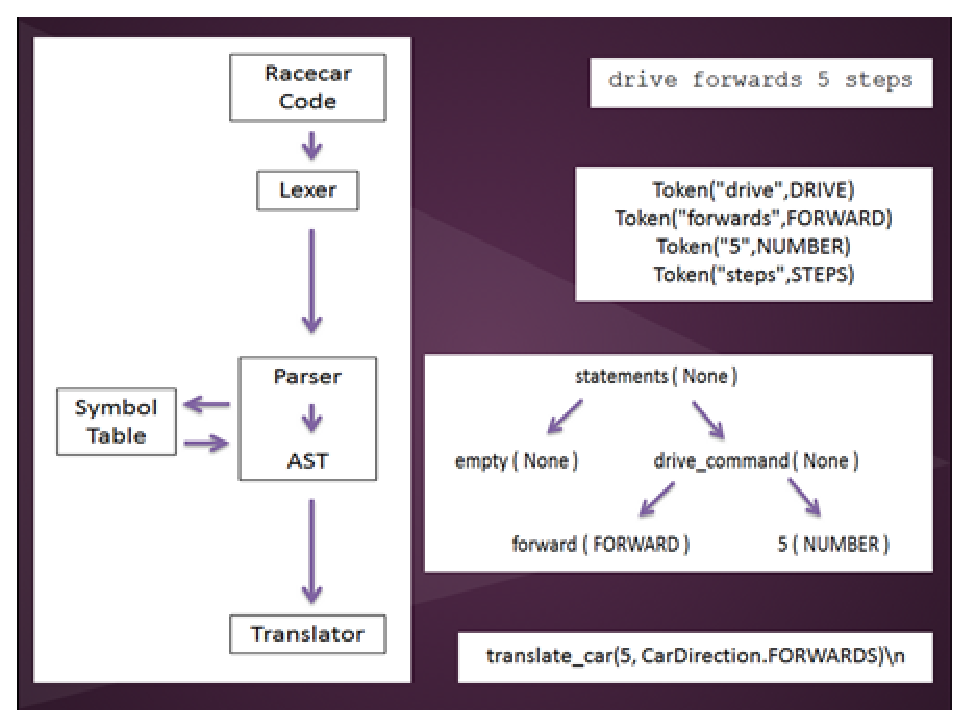
\includegraphics[width=1\textwidth]{architecture}\caption{System Architecture}


\end{figure}


Although each team member played a part in the construction and maintenance
of the implementation of the architecture, the following shows the
module and which team members had the most influential role in its
development:

Lexer(Sam Kohn) Parser-AST(Sam Kohn, Jeremy Spencer) Semantic Analyzer(Alex
Fields, Colfax Selby) Translator(Sam Kohn, Jeremy Spencer) IDE(Mason
Silber, Sam Kohn)


\section{Development and Run-Time Environment}


\subsubsection{By Mason Silber}

We developed our language in Python using standard text editors like
Vim and Sublime Text. We also heavily relied on git and Github for
version control; since each member of the team was working on a number
of things at once, we wanted to make sure that we didn\textquoteright{}t
step on anyone\textquoteright{}s toes when making changes, so having
a central repository for our code base was essential. Our Integrated
Development Environment (IDE) launches directly from a package, so
no makefile is required to write code in our language.

The runtime environment is a simple IDE customized for the Racecar
language and the targeted demographic. From the IDE\textquoteright{}s
menu bar, the user has the ability to save their code to files, and
to open previously saved files. The user can also place obstacles
on screen through which the car must navigate. The IDE has three main
components: the coding text area, the console, and the canvas on which
the racecar moves. Each of these components will be briefly discussed.

The coding text area takes up the left side of the IDE, and is where
users write their Racecar programs. Once the user has written the
code they would like to run, they press the \textquotedblleft{}Run
Code\textquotedblright{} button located directly below the coding
text area. Buttons are also available to clear the coding text area
and to reset the car\textquoteright{}s position. Once \textquotedblleft{}Run
Code\textquotedblright{} has been pressed, another button labeled
\textquotedblleft{}Stop Program\textquotedblright{} becomes available,
which will terminate the running program.

The console is more straightforward. It is used to display textual
information to the reader. If a user attempts to run a program with
errors, the errors are output to the console with information about
where the error can be found. It also lets the user know when a program
has begun to be executed, and when it has finished running. Additionally,
users can put print statements in their code; those print statements
get printed to the console.

The heart of the runtime environment is in the canvas. The canvas
is the area in which the car drives, but more importantly, it\textquoteright{}s
where users get to see visual output of their code. The car animates
across the screen, driving forward and turning. The canvas also holds
a number of obstacles, should the user desire them (to be selected
from the menu bar at the top of the IDE window). Obstacles from things
as simple as blocks to things as complex as mazes are displayed on
the canvas, and the user has the responsibility to write an algorithm
to navigate through these obstacle courses. If the car collides with
any of the obstacles, the car is reset to its original position and
the user has to start over.

All of these features are implemented within the IDE to provide a
self-contained, fully featured experience for users. No setup is required
besides opening the IDE. No interaction with external files is required
or necessary under any circumstances. The IDE provides the entire
platform on which Racecar algorithms can be run, thereby simplifying
the entire experience for students and teachers alike.


\section{Test Plan}


\subsubsection{By Colfax Selby}

We used a segmented and iterative testing methodology. As our compiler
matured, we built up out tests to test functionality from end to end,
to make sure that not only every part works fine by itself, but every
part of the compiler works with each other. 

We leveraged the power of the Python framework unittest to handle
the testing suite and keep everything organized and easy to run. Below
I will get into the details of how we planned and executed our tests.


\subsection{Segmented Testing}

We had different test classes for each part of the compiler (Semantic
Analyzer, Translator, etc). We within each class we tested individual
functionalities of the given part of the compiler, which I will explain
below. The segmented nature of our test suite allowed for us to test
specific parts of the compiler separately from everything else, therefore
allowing us to solely test the Translator when it was implemented
and do the same for other parts of the compiler. The test program
would indicate how many errors and failed tests there were per class,
so it was easy to tell which part of the compiler was causing problems. 

Our three test classes were: Symbol Table, Translator, and Semantic
Analyzer. We decided to test the Parser along with the Translator
and the Semantic Analyzer, with parser specific error messages, in
order to avoid rewriting many similar tests and utilizing the strategy
of code reuse. Additionally, as each individual part was tested and
working, we built up many of the tests to not only test their particular
part of the compiler, but to test more steps along the way. We did
this so that we would have as many tests as possible, testing as many
things as possible, to ensure that we would catch any errors that
may have occurred.


\subsection{Iterative Testing}

We also took an iterative approach to testing. Rather than writing
the whole compiler and then running tests at the end, we wrote tests
along the way to ensure that each part and each bit of functionality
was implemented properly. Each of the tests had descriptive names
(such as test\_function\_invocation\_with\_one\_parameter or test\_get\_car\_position)
so in the output, if a test did fail, we could tell exactly what wasn\textquoteright{}t
working.

An example test, followed by a detailed explanation, is below:

def test\_function\_invocation\_with\_two\_parameters(self): test\_string
= \textbackslash{} \textquotedbl{}\textquotedbl{}\textquotedbl{}define
turnLeftThenDriveStraight using numStepsTurn \textbackslash{} (number)
and numStepsDrive (number) \{ turn left drive forward numStepsTurn
steps turn right drive forward numStepsDrive steps \} turnLeftThenDriveStraight
5 10 \textquotedbl{}\textquotedbl{}\textquotedbl{} correct\_translation
= \textbackslash{} \textquotedbl{}\textquotedbl{}\textquotedbl{}def
turnLeftThenDriveStraight(numStepsTurn, numStepsDrive): rotate\_car(WheelDirection.LEFT)
translate\_car(numStepsTurn, CarDirection.FORWARDS) rotate\_car(WheelDirection.RIGHT)
translate\_car(numStepsDrive, CarDirection.FORWARDS) turnLeftThenDriveStraight(5,
10) \textquotedbl{}\textquotedbl{}\textquotedbl{} result = Compiler.getPythonCode(test\_string)
ast = Parser.parseString(test\_string)

saErrors = SemanticAnalyzer.analyzeStart(ast) self.assertEqual(len(saErrors),
0)

self.assertEqual(len(ast.errors), 0) self.assertEqual(result{[}0{]},
correct\_translation)

As you can see, this test checks the functionality of the parser,
semantic analyzer, and the translator. The test\_string is an example
code snippet in our Racecar language. It is then manually translated
and stored in correct\_translation. The test Racecar snippet is then
run through the parser, semantic analyzer, and then the translator.
The outputs of each of these steps is check to ensure that there are
no errors. Finally, the output of the translator is checked against
the manual translation of the code, and if all of the above match
as expected, the test passes. If any of the above do not function
as expected, the particular assertion fails, and the test fails with
a descriptive output.


\section{Conclusions}


\subsection{Lessons Learned as a Team}


\subsubsection{Successes}

Many aspects of our project went according to plan or better. The
most important of these, in our opinion, was our choice of implementation
language, Python. Although we decided on our implementation language
(Python or OCaml) relatively late because we could not decide which
would be more helpful, all of us are glad we chose Python. The language
never interfered with our design, and the issues we did run into during
implementation were generally resolved by making the code simpler.
That is, we tended to mess up when we tried to write un-Python-like
code, which indicates to us that we made the right decision. A second
organizational success was our decision to only loosely follow our
team roles. We were worried at the beginning of the project that some
people would get stuck with the less interesting tasks, and some people
with much more work than the others, so we explicitly resolved to
not strictly follow our team roles. This had the positive effect of
encouraging us to look at each other's code without being forced to
(by, for example, the project manager), since we did not have a one-to-one
correspondence between people and modules. This means that every module
has been read and approved by at least two people, yet this was accomplished
not as its own task, but rather as part of the natural development
process.


\subsubsection{Opportunities for Improvement}

Overall our project went very smoothly, but we did run into a few
issues along the way. The biggest issue our team ran into was adhering
to the timeline and completing all desired functionality on under
the constraints. We did a good job of designing our language with
a manageable scope, but as the semester progressed, we didn\textquoteright{}t
have time to completely a few bits of the functionality we wanted
to implement. This did not end up being an issue, though, because
we made sure to implement the core functionality early on, so just
auxilary things had to be cut. 

Secondly, not really an issue, but the TkInter Python GUI framework
gave us a bit of trouble. This, however, was not necessarily a function
of our team\textquoteright{}s organization, but rather a function
of it being a GUI framework, therefore being inherently difficult
to learn and use.

Lastly, we decided to develop our interpreter module by module, rather
than outlining the foundation of each module and building up the language,
full stack, along the way. This did not necessarily cause us any problems,
but is worth mentioning because we could have potentially run out
of time with before having a chance to develop a whole module. If
we developed the modules concurrently, building up the language as
we went, if we ran out of time we would only need to limit the scope
of the language, which is comparably much less severe of a problem
than missing an entire module.


\subsection{Lessons Learned by Each Team Member}


\subsubsection{Sam Kohn}

As project manager, I was responsible for keeping the project on schedule
and ensuring sufficient communication between project members. I learned
one major lesson from each of these responsibilities. For the first
one, I discovered very quickly that I was more concerned on a day-to-day
basis with the project's progress than the rest of the team, probably
because I was responsible for the project deliverables' on-time completion.
Practically speaking, this meant that I was more motivated to begin
work on the modules, and consequently I wrote the beginnings of most
of the project's modules. The work balanced out since other team members
were eager to work on the project as the deadlines approached and
the modules were still not complete. The second lesson I learned involves
communication. I was concerned at the beginning of the project that
I would be too overbearing as project manager, in that I would be
incessantly emailing the other project members and that they would
become annoyed with hearing from me. Sure enough, I found myself contacting
everyone often enough that I thought I was being too micromanaging.
However, based on recent conversations, I learned that I was wrong,
and that the communication frequency was appropriate and was welcomed
by the other members of our team. 


\subsubsection{Alex Fields}

I learned that it is important to choose carefully the language one
is about to write code in before beginning. There was a decent amount
of back and forth amongst our group regarding what we should code
in before we decided on Python, but this choice seemed to be well
worth it.

I learned about the importance of a test suite. Testing was never
something that I had done before in a program. I was in charge of
writing the Semantic Analyzer, so having the tests at my disposal
made my job quite a bit easier. In fact, my Semantic Analyzer failed
over half its tests the first time we ran it, and there were many
more iterations of coding and testing until it was complete.

I learned that meeting regularly can make a big difference in the
end result of a project. I was hesitant to agree that we needed to
meet as much as Sam wanted to meet when we began, but I am glad that
we did. It allowed us to not reach a time of panic in trying to complete
our compiler as I had heard many teams do.

Lastly, I learned that there is always something left to do in a project.
Every time we think we have completed something, a bug arises or we
remember something we left out. I guess the lesson to be learned from
that is plan for many more issues than you expect.


\subsubsection{Jeremy Spencer}

As system architect I learned the importance of modularization. Breaking
a large project into manageable parts is essential for simplicity
and clarity. Doing this abstraction early on and integrating the implementation
goals to the project plan/deliverables helped to keep everyone on
track. The cohesion of each module also made the language's maintenance
and expansion easier.


\subsubsection{Mason Silber}


\subsection{Advice for Future Teams}

We would highly recommend future teams use Python. As Sam said, \textquotedblleft{}Python
was the language through which I felt it was least necessary to think
about the rules of the language while coding.\textquotedblright{}
Python is, of course, Racecar for adults. That being said, the language
being created may look nothing like Python and a different language
may be more suitable to the development of that language.

We were satisfied with our decision to make our assigned roles flexible.
Having the roles made it easy for us to assign a task if no one immediately
volunteered to complete that task, but we were flexible enough to
allow everyone to jump around to different roles within the project.

We also would recommend at least a semi-regular meeting schedule.
Our team began work early and met regularly. This was key to our success.


\subsection{Suggestions for the Instructor}

We would like to frame our response in terms of which parts of the
course we felt were helpful to us for our project, and which were
not. We understand that there are important aspects of compiler design
that were not relevant to our particular project but are still worth
learning, so we intend this section to be more of a ranking of the
impact each topic would have on our project if it were dropped.


\subsubsection{Topics we would have liked to see}
\begin{itemize}
\item More in-depth coverage of semantic analysis (more than just type checking).
For example, common ways to keep track of a variable's scope and how
to check the appropriate number of function parameters. We knew enough
to figure these out on our own, but all of the other components of
the compiler received much more thorough treatments, both in class
and on the homeworks.
\item More examples of lambda calculus (even though it was not directly
related to our project). As you probably discovered in the days preceding
the final exam, there was a lot of confusion about normal vs. applicative
order evaluation. Although explanations are helpful to an extent,
what really would have been great was a list of 3 or 4 lambda expressions
with step-by-step evaluations in both normal and applicative order.
We could not find good examples online.
\end{itemize}

\subsubsection{Topics that directly helped our project}
\begin{itemize}
\item Lexers
\item Common grammar patterns for compilers
\item Bottom-up parsing
\item Synthetic syntax-directed definitions and translations
\end{itemize}

\subsubsection{Topics that did not help our project, but maybe helped other projects}
\begin{itemize}
\item Lambda Calculus
\item Types and type-checking
\end{itemize}

\subsubsection{Topics that did not help our project or seem relevant to any project}
\begin{itemize}
\item Top-down parsing. Everyone was advised to use yacc, which uses bottom-up
parsing.
\item Inherited syntax-directed translation. Again, this would only be useful
in top-down parsing.
\item Three address codes
\item Code optimizations
\end{itemize}

\section{Appendix}
\end{document}
